\Chapter{Introduction}
{For thousands of years, the Tablelands have remained untouched: its politics frozen in a delicate stalemate, its life in a balance even more delicate. It is true that the Dragon Kings amused themselves with their petty wars, rattling sabers to punctuate the passing of ages. It is true that, occasionally, another city would be swallowed by the wastes.

But there were no surprises. The Dragon Kings steered everything from their omnipotent perches, content in their superiority, but ever thirsting for challenge. All that has changed. The Tablelands have been thrown into turmoil, the likes of which have not been seen since times forgotten. The Dragon Kings have been thrown into confusion, grasping for the tedium they so recently lamented.

And yet I fear the worst is yet to come. Change is in the air, and change has never come gently to Athas.}{Oronis, sorcerer-king of Kurn}

\begin{figure*}[b!]
\centering
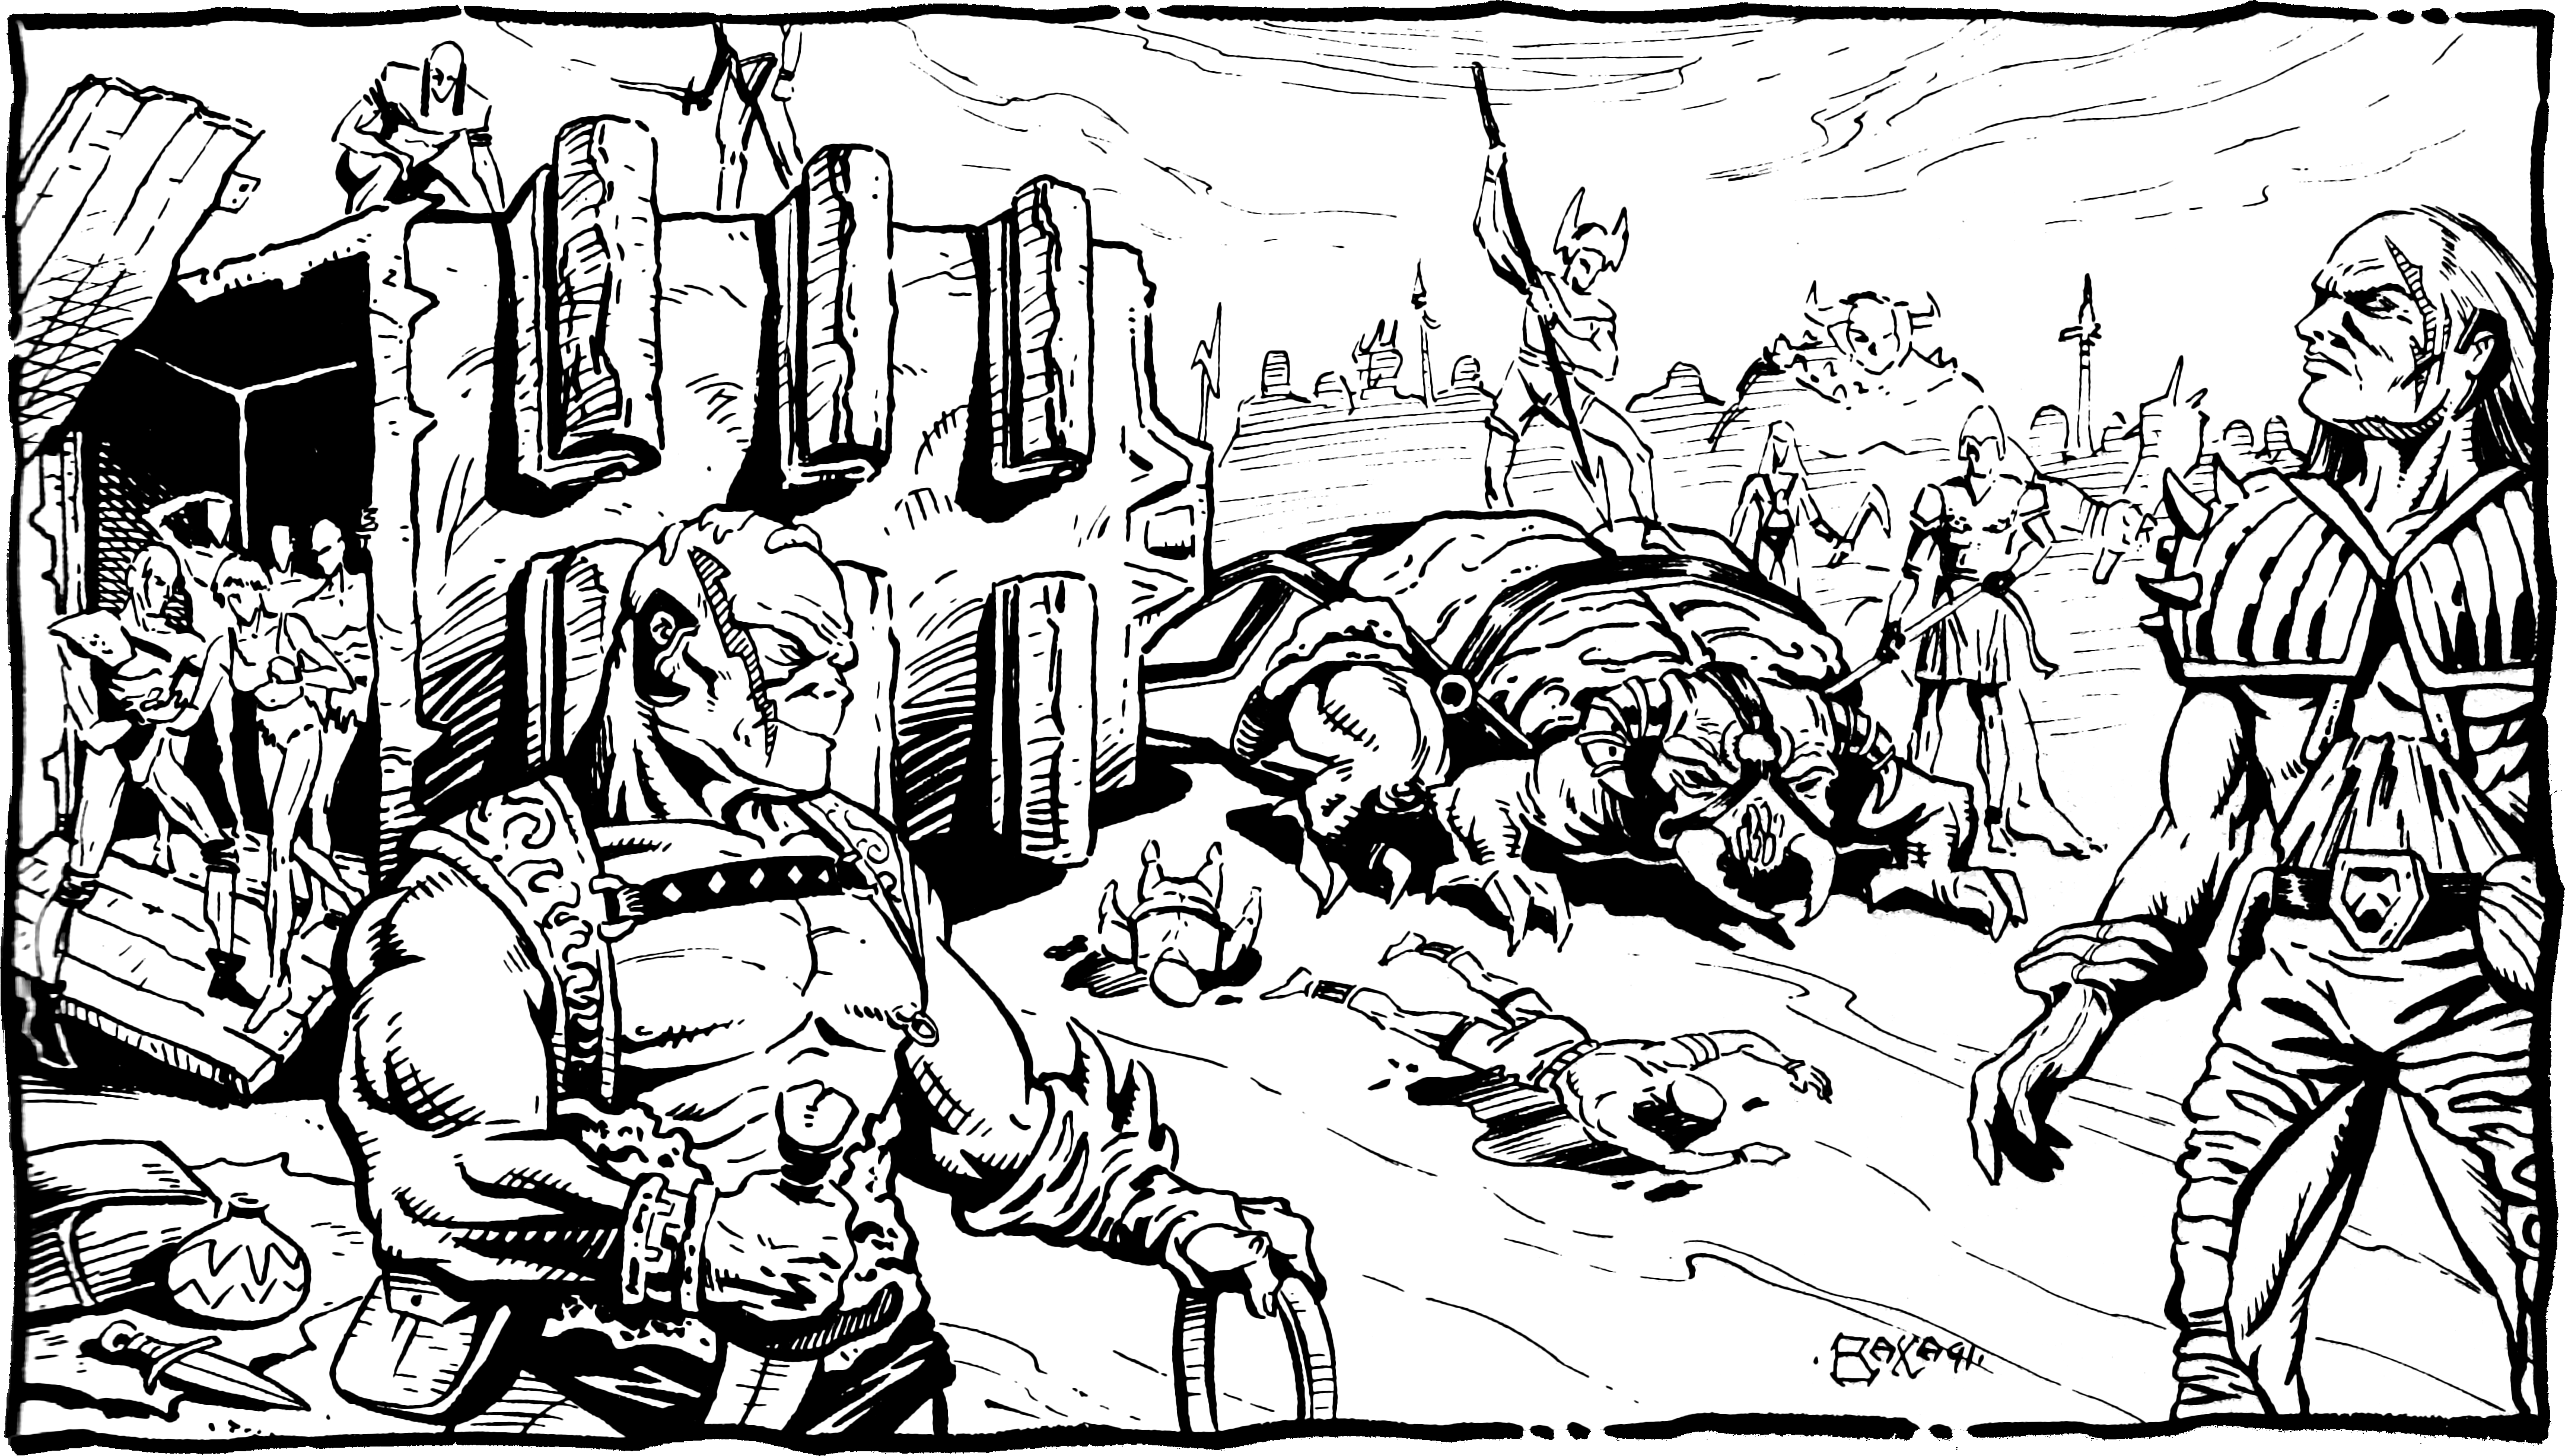
\includegraphics[width=\textwidth-1cm]{images/raiders-2.png}
\WOTC
\end{figure*}

\Capitalize{D}{ark} Sun 3.5 is a new edition of the {\tableheader Dark Sun} campaign setting, written as a revision of athas.org's {\tableheader Dark Sun} 3 rulebook and the Athasian Emporium. This rulebook condenses all d20 System information available under OGL, including psionic rules, but it also changes the system a bit, getting inspiration on the 5th edition by adding advantage and multiclass prerequisites. In addition, you might find useful to download the Terrors of Athas (ToA), Terrors of the Dead Lands (TotDL), and Faces of the Forgotten North (FFN), since this book does not contain information on monsters.

This document is intended for an audience already familiar with the {\tableheader Dark Sun} campaign setting, and does not attempt to detail the world of Athas in full. For more information on Athas, visit \url{www.athas.org}---the official {\tableheader Dark Sun} website. In addition to the latest version of this document, you may find other {\tableheader Dark Sun} material available as free downloads.

All {\tableheader Dark Sun} products published by TSR may be purchased from RPGNow! as PDF downloads.

\section{This is Athas}
Athas' savage, primal landscape is the result of long centuries of ecological and magical abuses. The world is dying. It breathes its last gasps as water turns to silt, grasslands become sandy wastes, and jungles decay into stony barrens. Still, life finds ways to endure even in these hellish conditions. In fact, it thrives.

Children growing up beneath the crimson sun don't aspire to become heroes. True heroes who champion causes or seek to make the world a better place are as rare as steel on Athas. Living to see the next dawn is more important than defending a set of beliefs, so survival ultimately motivates all living creatures---not virtue or righteousness.

But heroes are desperately needed in tfhis harsh, savage world... Heroes like the ones who stepped forward to destroy the sorcerer-king Kalak and set Tyr free. Heroes like those who risked everything to kill the Dragon and keep Rajaat the Warbringer from devastating the land.

Today, Athas rushes toward its future. If the course of destruction is to be diverted, of Athas is to be restored, then more heroes must grab the reins of destiny and give new hope and promise to the world.

\section{Ten Things You Need to Know}
Every Dungeon Master and player needs to know and remember these facts about the world of Athas.

\begin{enumerate}
\item \textbf{{\tableheader Dark Sun} is Different from Traditional D\&D.} Many monsters, prestige classes, spells or magic items from the core rulebooks simply are not available in Athas. Many races were extinguished from Athas during the Cleansing Wars. This is because Athas has a very different background than most D\&D settings. Check with your DM to see which options you have to choose from before building your character.

\item \textbf{Tone and Attitude.} Athas puts the survival of the fittest concept to its fullest. Those who cannot adapt to endure the tyrannical sorcerer-kings, the unrelenting sun, or the many dangers of the wastes will certainly perish. Illiteracy and slavery are commonplace, while magic is feared and hated. The term ``hero'' has a very different meaning on Athas.

\item \textbf{A Burnt World.} Thousands of years of reckless spellcasting and epic wars have turned Athas into a barren world, on the verge of an ecological collapse. From the first moments of dawn until the last twinkling of dusk, the crimson sun shimmers in the olive-tinged sky like a fiery puddle of blood, creating temperatures up to 65$^\circ$ C (150$^\circ$ F) by late afternoon. Waters is scarce, so most Athasians need to come up with alternative solutions for dealing with the heat or perish.

\item \textbf{A World Without Metal.} Metals are very rare on Athas. Its scarcity has forced Athasians to rely on barter and different materials, such as ceramic, to use as currency. It also hampers industrial and economic development as well; mills and workshops rarely have quality tools to produce everyday products. Even though most Athasians have developed ways of creating weapons and armor made of nonmetallic components, but the advantage of having metal equipment in battle is huge.

\item \textbf{The Will and The Way.} From the lowliest slave to the most powerful sorcerer-king, psionics pervade all levels of Athasian society. Virtually every individual has some mental ability, and every city-state has some sort of psionic academy available. Athasians use the term Will to refer to someone's innate ability for psionics and the Way for the study of psionics.

\item \textbf{A World Without Gods.} Athas is a world without true deities. Powerful sorcerer-kings often masquerade as gods but, though their powers are great and their worshipers many, they are not true gods. Arcane magic require life force, either from plants or animals, to be used. All divine power comes from the Elemental planes and the spirits of the land that inhabit geographic features.

\item \textbf{Planar Insulation.} Barriers exist between Athas and other planes. In the case of other planes of existence, the Gray impedes planar travel, except to the Elemental Planes. Consequently, travel via spelljamming is impossible, and planar travel is much more difficult. The same holds true for those trying to contact or reach Athas. The barrier formed by the Gray impedes travel in both directions.

\item \textbf{The Struggle For Survival.} The basic necessities of life are scarce on Athas. This means that every society must devote itself to attaining food and safeguarding its water supply, while protecting themselves from raiding tribes, Tyr-storms, and other city-states. This essentially means that most Athasian must devout a large deal of their lives just to survive.

\item \textbf{The Seven City-states.} The Tyr Region is the center of the world of Athas, at least as far as the people of the seven city-states are concerned. It's here, along the shores of the Silt Sea and in the shadows of the Ringing Mountains that civilization clings to a few scattered areas of fertile land and fresh water. The majority of the population lives in the city-states of Tyr, Urik, Raam, Draj, Nibenay, Gulg, and Balic. The remainder lives in remote villages built around oases and wells, or wanders about in nomadic tribes searching for what they need to survive.

\item \textbf{New and Changed Races.} The common races found in D\&D changed with the harsh planet, elves are tireless nomads, dwarves are bald and have a focused mind, half-elves struggle to fit in the society, and halflings are cannibals living in the jungles. In addition to those races, players can choose to play aarakocra, half-giants, muls, pterrans, and thri-kreen. Aarakocra are avian freedom-loving creatures, but extremely zealous and xenophobic. Half-giants are creatures with great strength, but dull wits. Muls are a hybrid race that combines the natural dwarven resilience and stubbornness with the adaptability from humans. Pterrans are reptilian nature-worshiping creatures that are always in the pursuit of their ``life paths''. Thri-kreen are insectoid creatures that roam the Athasian wastes in search for prey.
\end{enumerate}

\section{The Five Ages of Play}
{\tableheader Dark Sun} 3 supports adventures and campaigns set in many different ages, five of which are detailed in this book. You can set your campaign right after the events of the Prism Pentad. Known as the Age of Heroes, this is a period that fundamentally changed the world, when individuals begun fighting back all the tyranny and oppression, ending up with several sorcerer-kings dead and the first free city of the Tablelands appeared.

Or, you can go backward in time to the classic period where most sorcerer-kings were still alive and play during the Brown Age or the Age of Sorcerer-kings, when the world was becoming more and more a wasteland by defiling magic, and the Dragon of Tyr was almighty.

Or, you can go even more backward in time and play during the Cleansing Wars, when Rajaat unleashed his human armies and his Champions in order to wipe out all other intelligent races from the face of Athas.

Or, you can go to Green Age, when the New Races began populating the lands left unscathed by the receding waves, and the first great cities were found, and psionics started to show its true power.

Or, you can go to the very first age, known as the Blue Age, when the world was still young and the only intelligent races where the rhulisti, the ancient halflings, and the kreen, lived in a world filled with oceans and a blue sun, and magic was nonexistent.

In addition, the rules set in this book can be used to support campaigns set in other ages. For example, you could forward to several hundred years into the future, in a world that could be either devastated by the Kreen invasion, or that has just begun to heal from most of the damage it suffered since Rajaat discovered arcane magic. Although these ages are not covered in this book, the rules herein can be used as a basis for play in them.

\section{Where to Begin}
Players should begin by creating their {\tableheader Dark Sun} character after reading the first seven chapters of this book. Players may also want to read the timeline in order to understand the history of Athas. Remember to discuss with your DM before creating your character to find out what options and other books are allowed in his campaign.

The DM should start with \chapref{Life on Athas} and read material relevant to the locations, \chapref{Athasian Campaigns} for guidelines and tips when running your campaign, and \chapref{Others Eras of Play} to understand more about the era of play on which your campaign will focus.

\begin{figure}[t!]
\centering
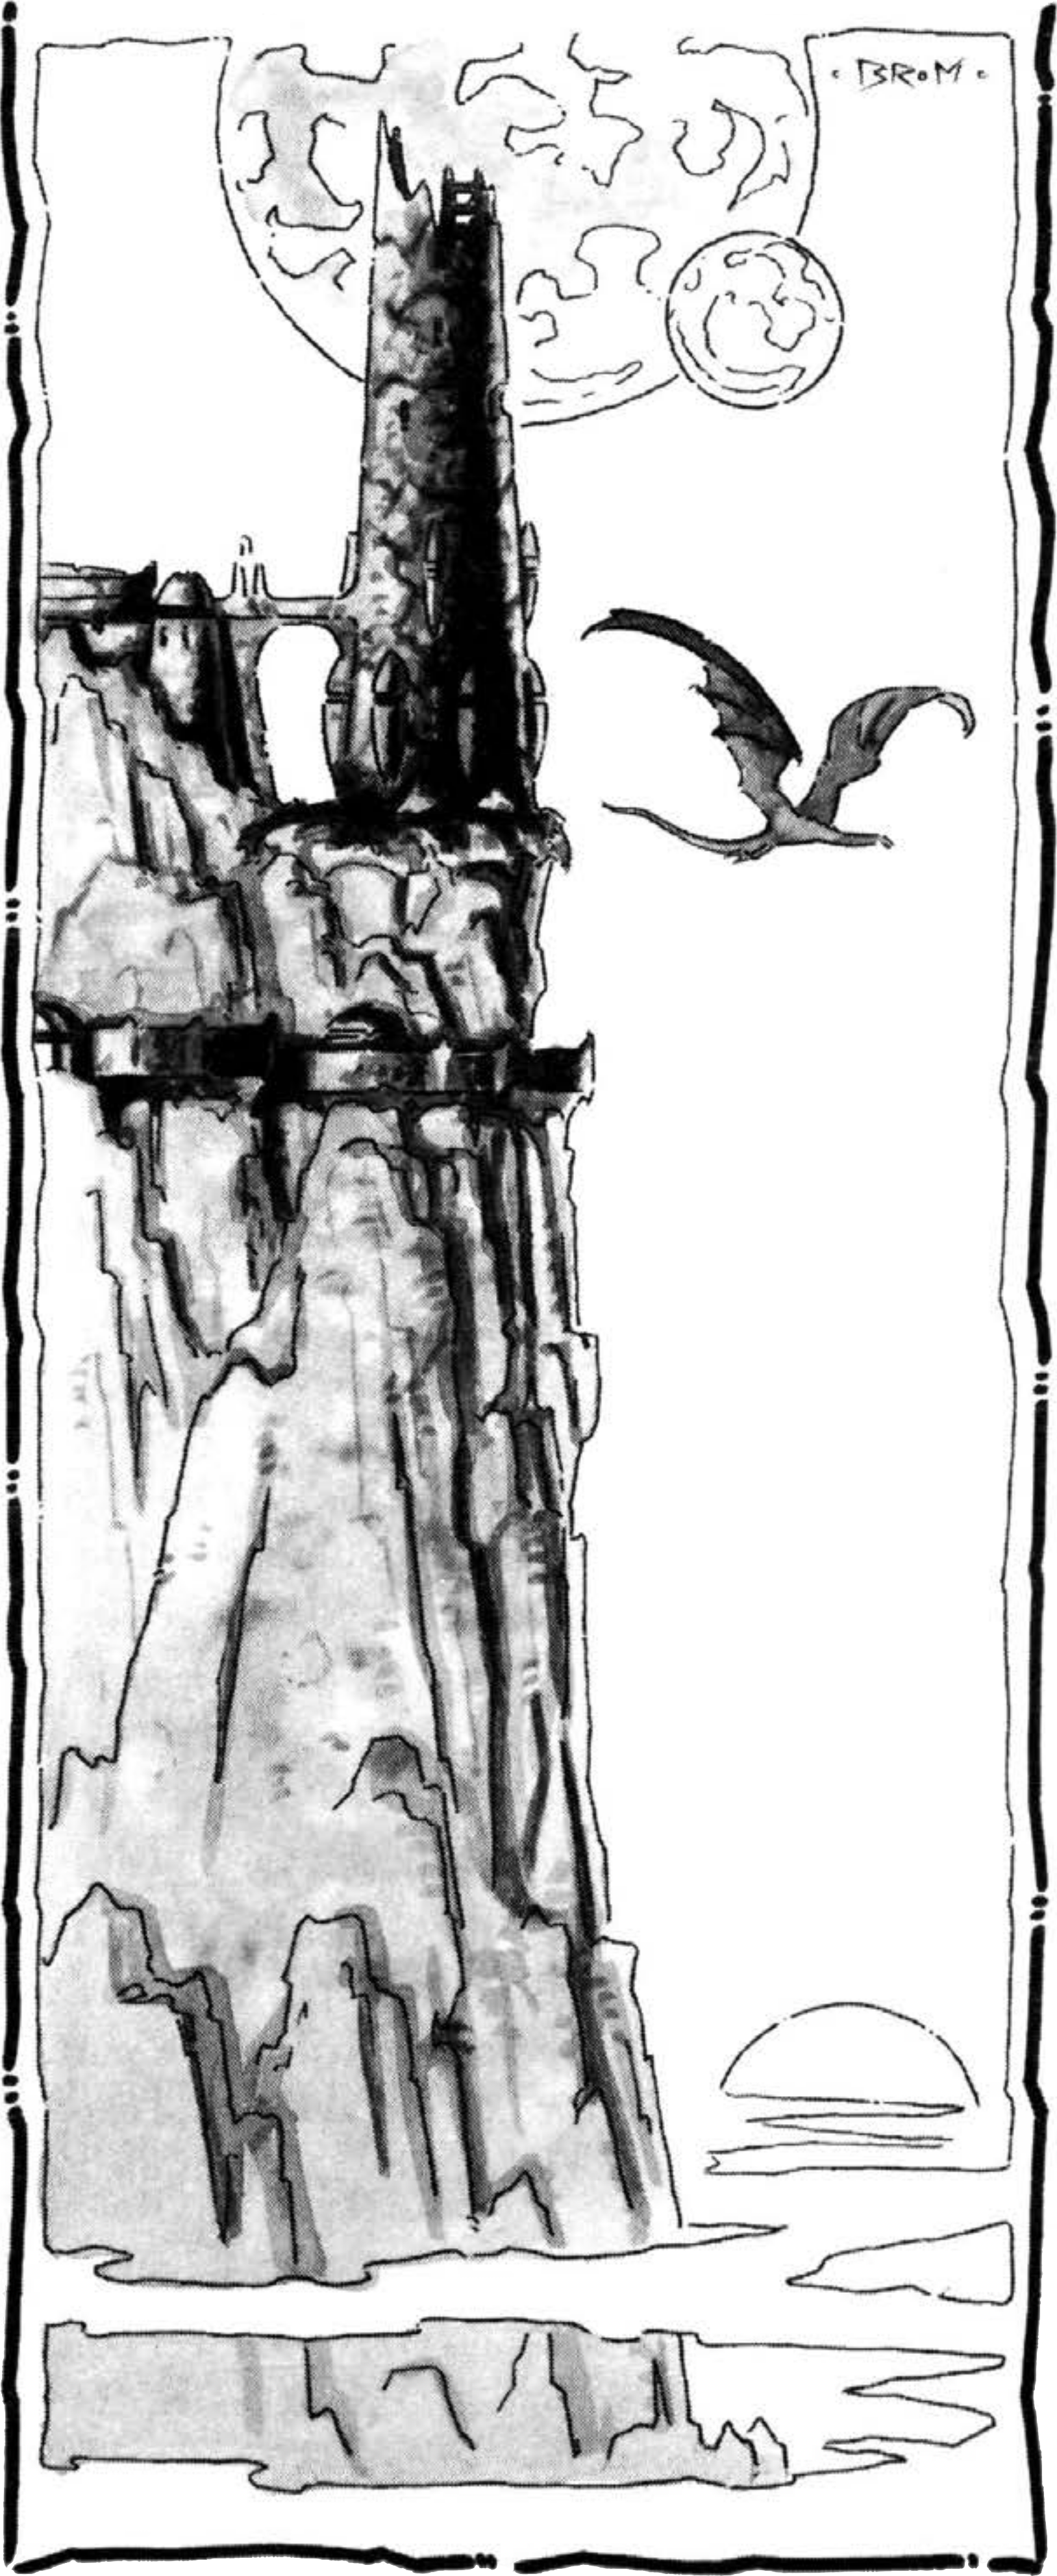
\includegraphics[width=\columnwidth-8mm]{images/tower-1.png}
\WOTC
\end{figure}


\begin{figure*}[b!]
\centering
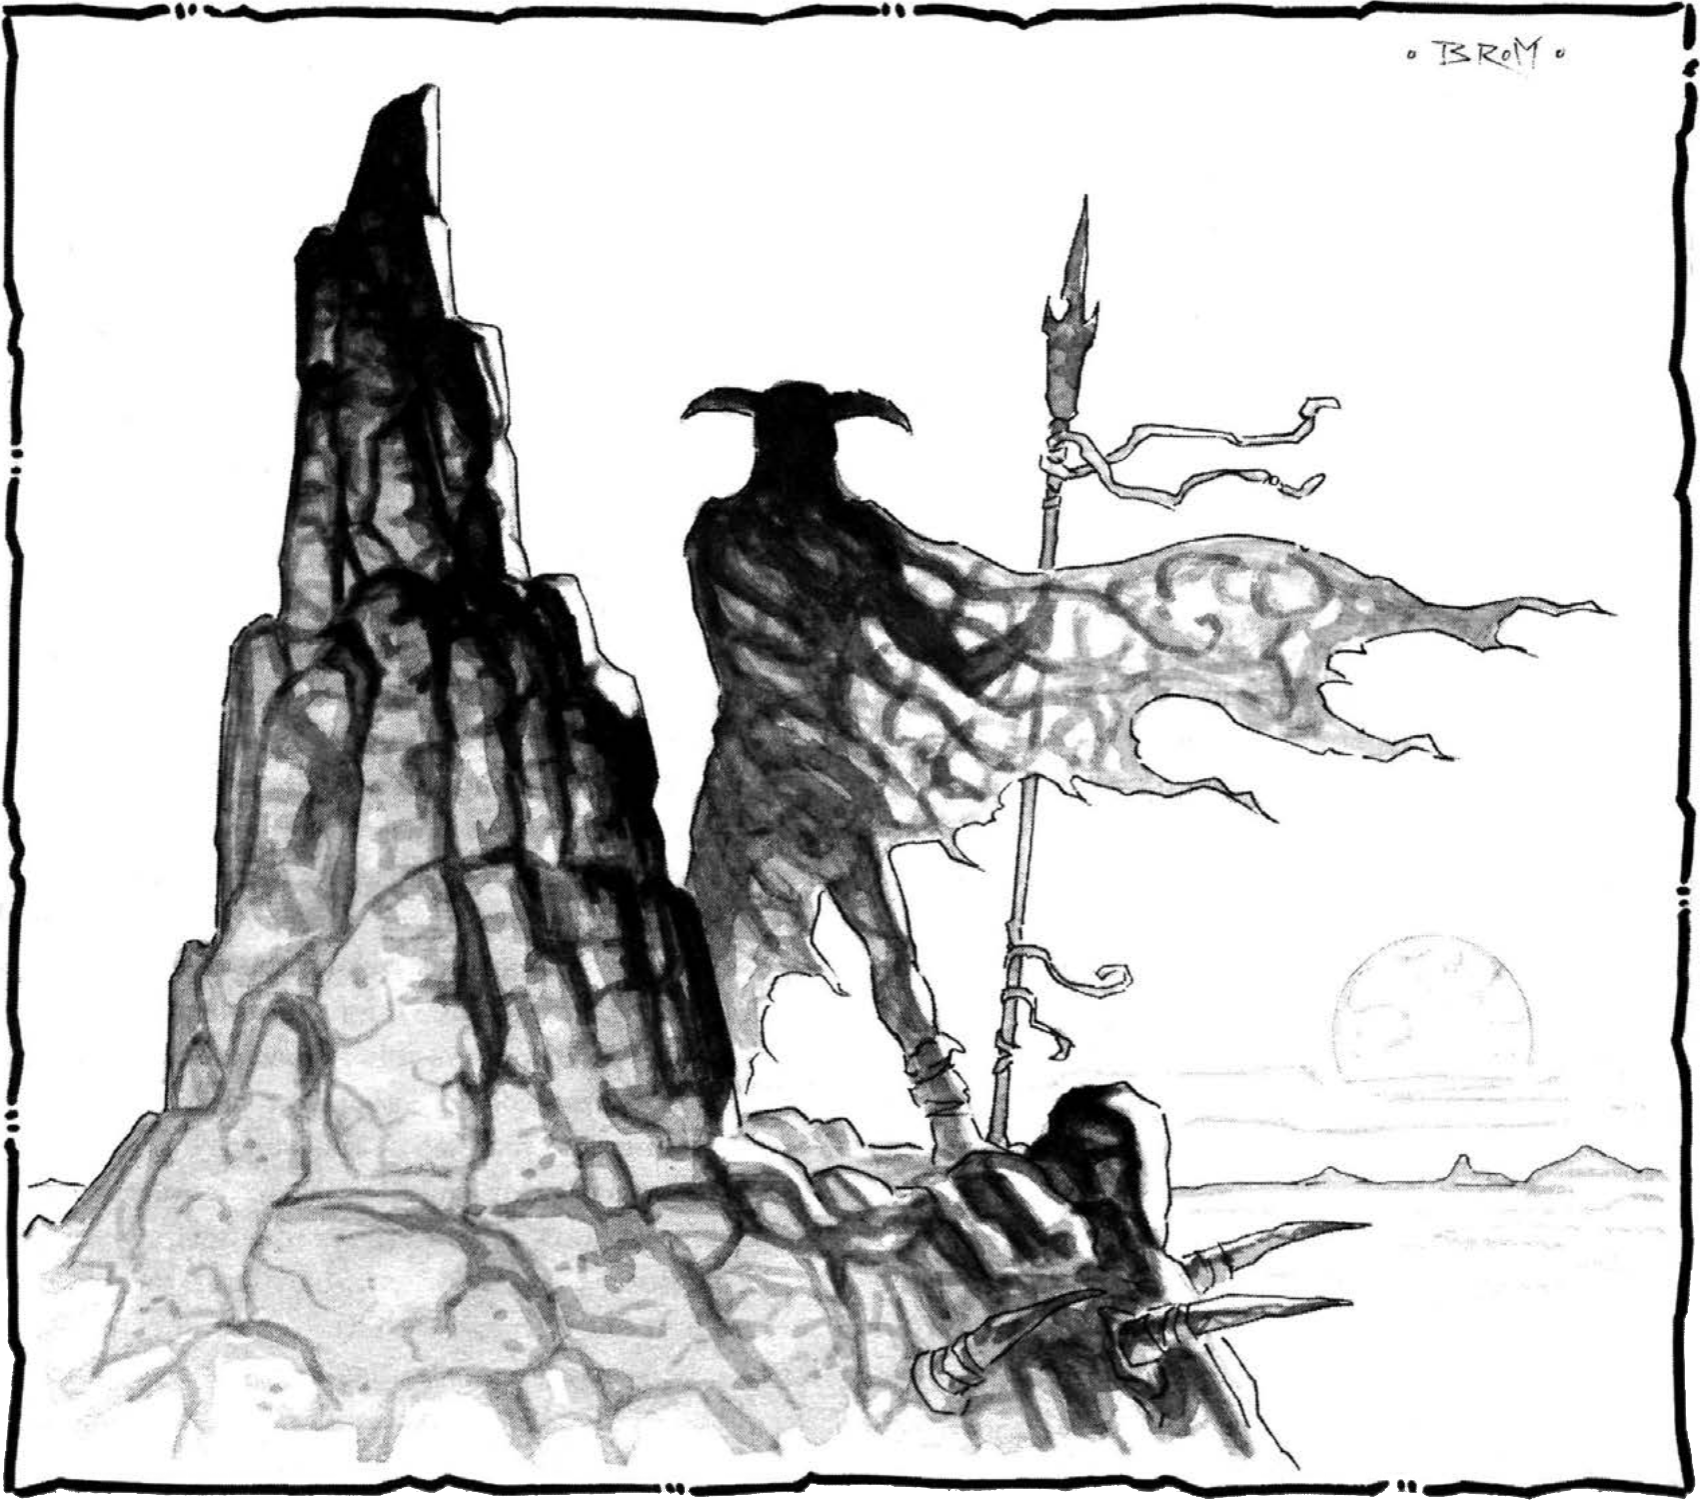
\includegraphics[width=\textwidth-5mm]{images/adventurer-2.png}
\WOTC
\end{figure*}

\section{The Core Mechanic}
Whenever you attempt an action that has some chance of failure, you roll a twenty-sided die (d20). To determine if your character succeeds at a task you do this:

\begin{itemize*}
\item Roll a d20.
\item Add any relevant modifiers.
\item Compare the result to a target number.
\item If the result equals or exceeds the target number, your character succeeds. If the result is lower than the target number, you fail.
\end{itemize*}

\subsection{Dice}
Dice rolls are described with expressions such as ``3d4+3,'' which means ``roll three four-sided dice and add 3'' (resulting in a number between 6 and 15). The first number tells you how many dice to roll (adding the results together). The number immediately after the ``d'' tells you the type of die to use. Any number after that indicates a quantity that is added or subtracted from the result.

\textbf{d\%:} Percentile dice work a little differently. You generate a number between 1 and 100 by rolling two different ten-sided dice. One (designated before you roll) is the tens digit. The other is the ones digit. Two 0s represent 100.

\subsection{Modifiers}
A modifier is any bonus or penalty applying to a die roll. A positive modifier is a bonus, and a negative modifier is a penalty.

\subsubsection{Stacking}
In most cases, modifiers to a given check or roll stack (combine for a cumulative effect) if they come from different sources and have different types (or no type at all), but do not stack if they have the same type or come from the same source (such as the same spell cast twice in succession). If the modifiers to a particular roll do not stack, only the best bonus and worst penalty applies. Dodge bonuses and circumstance bonuses however, do stack with one another unless otherwise specified.

\subsubsection{Modifier Types}
\textbf{Ability Modifier:} The bonus or penalty associated with a particular ability score. Ability modifiers apply to die rolls for character actions involving the corresponding abilities.

\textbf{Alchemical Bonus:} An alchemical bonus is granted by the use of a nonmagical, alchemical substance such as antitoxin.

\textbf{Armor Bonus:} An armor bonus applies to Armor Class and is granted by armor or by a spell or magical effect that mimics armor. Armor bonuses stack with all other bonuses to Armor Class (even with natural armor bonuses) except other armor bonuses. An armor bonus doesn't apply against touch attacks, except for armor bonuses granted by force effects (such as the mage armor spell) which apply against incorporeal touch attacks, such as that of a shadow.

\textbf{Circumstance Modifier:} A circumstance bonus (or penalty) arises from specific conditional factors impacting the success of the task at hand. Circumstance bonuses stack with all other bonuses, including other circumstance bonuses, unless they arise from essentially the same source.

\textbf{Competence Modifier:} A competence bonus (or penalty) affects a character's performance of a particular task, as in the case of the bardic ability to inspire competence. Such a bonus may apply on attack rolls, saving throws, skill checks, caster level checks, or any other checks to which a bonus relating to level or skill ranks would normally apply. It does not apply on ability checks, damage rolls, initiative checks, or other rolls that aren't related to a character's level or skill ranks. Multiple competence bonuses don't stack; only the highest bonus applies.

\textbf{Deflection Bonus:} A deflection bonus affects Armor Class and is granted by a spell or magic effect that makes attacks veer off harmlessly. Deflection bonuses stack with all other bonuses to AC except other deflection bonuses. A deflection bonus applies against touch attacks.

\textbf{Dodge Bonus:} A dodge bonus improves Armor Class (and sometimes Reflex saves) resulting from physical skill at avoiding blows and other ill effects. Dodge bonuses are never granted by spells or magic items. Any situation or effect (except wearing armor) that negates a character's Dexterity bonus also negates any dodge bonuses the character may have. Dodge bonuses stack with all other bonuses to AC, even other dodge bonuses. Dodge bonuses apply against touch attacks.

\textbf{Enhancement Bonus:} An enhancement bonus represents an increase in the sturdiness and/or effectiveness of armor or natural armor, or the effectiveness of a weapon, or a general bonus to an ability score. Multiple enhancement bonuses on the same object (in the case of armor and weapons), creature (in the case of natural armor), or ability score do not stack. Only the highest enhancement bonus applies. Since enhancement bonuses to armor or natural armor effectively increase the armor or natural armor's bonus to AC, they don't apply against touch attacks.

\textbf{Insight Bonus:} An insight bonus improves performance of a given activity by granting the character an almost precognitive knowledge of what might occur. Multiple insight bonuses on the same character or object do not stack. Only the highest insight bonus applies.

\textbf{Luck Modifier:} A luck modifier represents good (or bad) fortune. Multiple luck bonuses on the same character or object do not stack. Only the highest luck bonus applies.

\textbf{Morale Modifier:} A morale bonus represents the effects of greater hope, courage, and determination (or hopelessness, cowardice, and despair in the case of a morale penalty). Multiple morale bonuses on the same character do not stack. Only the highest morale bonus applies. Nonintelligent creatures (creatures with an Intelligence of 0 or no Intelligence at all) cannot benefit from morale bonuses.

\textbf{Natural Armor Bonus:} A natural armor bonus improves Armor Class resulting from a creature's naturally tough hide. Natural armor bonuses stack with all other bonuses to Armor Class (even with armor bonuses) except other natural armor bonuses. Some magical effects (such as the barkskin spell) grant an enhancement bonus to the creature's existing natural armor bonus, which has the effect of increasing the natural armor's overall bonus to Armor Class. A natural armor bonus doesn't apply against touch attacks.

\textbf{Profane Modifier:} A profane bonus (or penalty) stems from the power of evil. Multiple profane bonuses on the same character or object do not stack. Only the highest profane bonus applies.

\textbf{Racial bonus:} A bonus granted because of the culture a particular creature was brought up in or because of innate characteristics of that type of creature. If a creature's race changes (for instance, if it dies and is reincarnated), it loses all racial bonuses it had in its previous form.

\textbf{Resistance Bonus:} A resistance bonus affects saving throws, providing extra protection against harm. Multiple resistance bonuses on the same character or object do not stack. Only the highest resistance bonus applies.

\textbf{Sacred Modifier:} A sacred bonus (or penalty) stems from the power of good. Multiple sacred bonuses on the same character or object do not stack. Only the highest sacred bonus applies.

\textbf{Shield Bonus:} A shield bonus improves Armor Class and is granted by a shield or by a spell or magic effect that mimics a shield. Shield bonuses stack with all other bonuses to AC except other shield bonuses. A magic shield typically grants an enhancement bonus to the shield's shield bonus, which has the effect of increasing the shield's overall bonus to AC. A shield bonus granted by a spell or magic item typically takes the form of an invisible, tangible field of force that protects the recipient. A shield bonus doesn't apply against touch attacks.

\textbf{Size Modifier:} A size bonus or penalty is derived from a creature's size category. Size modifiers of different kinds apply to Armor Class, attack rolls, Hide checks, grapple checks, and various other checks.

\subsubsection{Rounding Fractions}
In general, if you wind up with a fraction, round down, even if the fraction is one-half or larger.

\textit{Exception:} Certain rolls, such as damage and hit points, have a minimum of 1.

\begin{figure*}[b!]
\centering
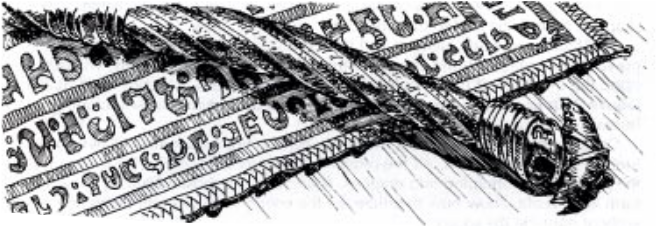
\includegraphics[width=\textwidth]{images/filler-1.png}
\WOTC
\end{figure*}

\subsection{Multiplying}
Sometimes a rule makes you multiply a number or a die roll. As long as you’re applying a single multiplier, multiply the number normally. When two or more multipliers apply to any abstract value (such as a modifier or a die roll), however, combine them into a single multiple, with each extra multiple adding 1 less than its value to the first multiple. Thus, a double ($\times$2) and a double ($\times$2) applied to the same number results in a triple ($\times$3, because 2 + 1 = 3).

\vskip1cm

When applying multipliers to real-world values (such as weight or distance), normal rules of math apply instead. A creature whose size doubles (thus multiplying its weight by 8) and then is turned to stone (which would multiply its weight by a factor of roughly 3) now weighs about 24 times normal, not 10 times normal. Similarly, a blinded creature attempting to negotiate difficult terrain would count each square as 4 squares (doubling the cost twice, for a total multiplier of $\times$4), rather than as 3 squares (adding 100\% twice).

\subsection{Advantage and Disadvantage}
Sometimes a special ability or spell tells you that you have advantage or disadvantage on an ability check, a saving throw, or an attack roll. When that happens, you roll a second d20 when you make the roll. Use the higher of the two rolls if you have advantage, and use the lower roll if you have disadvantage. For example, if you have disadvantage and roll a 17 and a 5, you use the 5. If you instead have advantage and roll those numbers, you use the 17.

If multiple situations affect a roll and each one grants advantage or imposes disadvantage on it, you don’t roll more than one additional d20. If two favorable situations grant advantage, for example, you still roll only one additional d20.

If circumstances cause a roll to have both advantage and disadvantage, you are considered to have neither of them, and you roll one d20. This is true even if multiple circumstances impose disadvantage and only one grants advantage or vice versa. In such a situation, you have neither advantage nor disadvantage.